\section{Local Asymmetry in the Dalitz Plane}
\label{sec:dalitz}
\label{sec:bayes_dalitz}
\emph{In short: the asymmetry is not uniform over the Dalitz plane ($\chi^2=80.8$ for $31$ degrees of freedom); it is concentrated at low $m^2_{\mathrm{lo}}$ outside the $\phi(1020)$ and, in the region of the published analysis of the same data, it reproduces the published value.}
To test whether the asymmetry is uniform over phase space or concentrated in specific regions, each candidate was placed in the Dalitz plane using the two opposite-sign $K^+K^-$ invariant masses $m^2(H1,H2)$ and $m^2(H1,H3)$ (Sec.~\ref{sec:data_presel}), sorted into $m^2_{\mathrm{lo}}$ and $m^2_{\mathrm{hi}}$ to remove the $H2/H3$ labeling ambiguity. The plane $[0,16]\times[0,30]\,\GeV^2$ in $(m^2_{\mathrm{lo}},m^2_{\mathrm{hi}})$ was divided into an $8\times8$ grid, fixed before looking at the asymmetries. In each bin with at least 20 candidates (32 of 64), the local asymmetry $A_i=(N_i^--N_i^+)/N_i$, with binomial uncertainty $\sigma(A_i)=\sqrt{(1-A_i^2)/N_i}$, was compared with the global counting asymmetry $A_{\mathrm{glob}}=-0.043$ through $S_i=(A_i-A_{\mathrm{glob}})/\sigma(A_i)$.

\begin{figure*}[t]
\centering
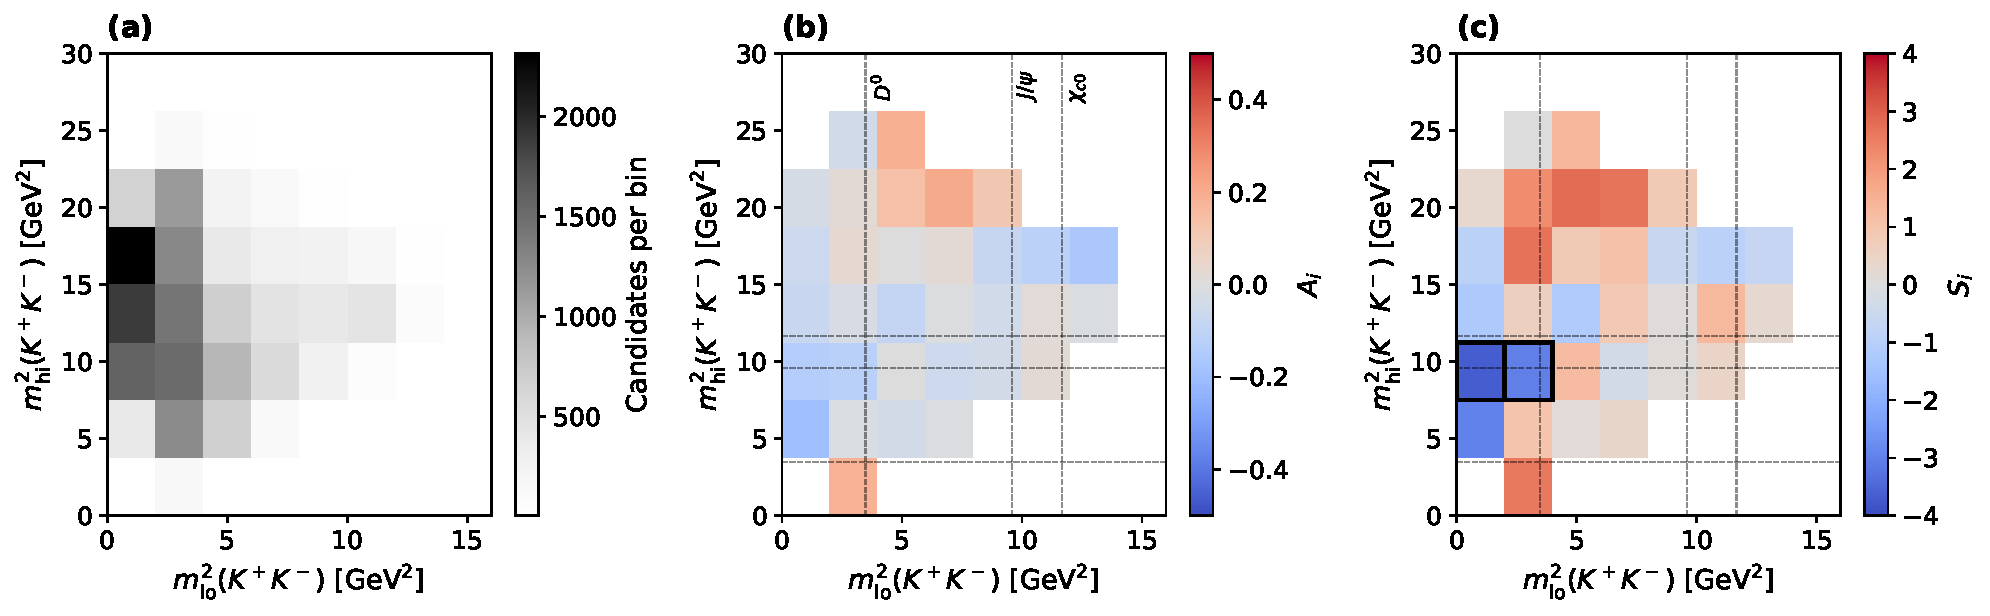
\includegraphics[width=0.95\textwidth]{figures/bayes_nominal_dalitz_maps.pdf}
\caption{Fixed $8\times8$ Dalitz-plot binning, all candidates in the fit window: (a) number of candidates per bin, (b) local asymmetry $A_i$ for bins with $\geq20$ candidates, and (c) local significance with respect to the global asymmetry, $(A_i-A_{\mathrm{glob}})/\sigma(A_i)$. The two bins with $|S_i|>3$ are outlined. Dashed lines: the squared masses of the $D^0$, $J/\psi$ and $\chi_{c0}$, in either opposite-sign pair.}
\label{fig:bayes_dalitz}
\end{figure*}

Figure~\ref{fig:bayes_dalitz} shows the occupancy of the bins (a), the local asymmetry (b) and its significance (c). Two of the 32 bins have $|S_i|>3$, adjacent at $m^2_{\mathrm{lo}}<4\,\GeV^2$ and $7.5<m^2_{\mathrm{hi}}<11.25\,\GeV^2$ ($S_i=-3.7$ and $-3.0$); about $0.09$ such bins would be expected if the asymmetry were uniform, and two or more with probability $3\times10^{-3}$, a look-elsewhere number over any two of the 32 bins. The global homogeneity test, $\chi^2=\sum_iS_i^2=80.8$ for 31 degrees of freedom ($p=3\times10^{-6}$), confirms that the local asymmetry is not uniform; it also holds in the signal window alone, with the charm vetoes and for other grids (Appendix~\ref{app:ext_dalitz}).

Two null tests check the procedure itself. Shuffling the charges among the candidates removes any local asymmetry while keeping the occupancy of the bins and the global asymmetry of the data: over $2000$ permutations the $8\times8$ grid gives $\chi^2=31.5\pm8.4$, as expected for 31 degrees of freedom, and no permutation reaches the observed value (permutation $p<5\times10^{-4}$; $p=1\times10^{-3}$ for the $12\times12$ grid). The phase-space simulation of the record, without asymmetry by construction, gives $\chi^2=40.0/30$ ($p=0.11$) with the same procedure on the whole sample; on $500$ subsamples of the size of the data the mean $\chi^2/\mathrm{ndof}$ is $1.16$ and $13\%$ have $p<0.05$, so the $\chi^2$ $p$-values are slightly optimistic (the binomial uncertainty is evaluated at the observed $A_i$). The permutation test, whose null distribution is exact, gives the same conclusion: the non-uniformity is a property of the data.

The structure is the same with both magnet polarities: in the region of the two significant bins the counting asymmetry is $-0.129\pm0.023$ (magnet down) and $-0.126\pm0.028$ (magnet up), and the two maps agree bin by bin ($\chi^2=23.0$ for 29 bins, $p=0.78$). The split tests the part of the detection asymmetry that changes sign with the polarity, not the different interaction of $K^+$ and $K^-$ with the detector material.

\begin{figure*}[t]
\centering
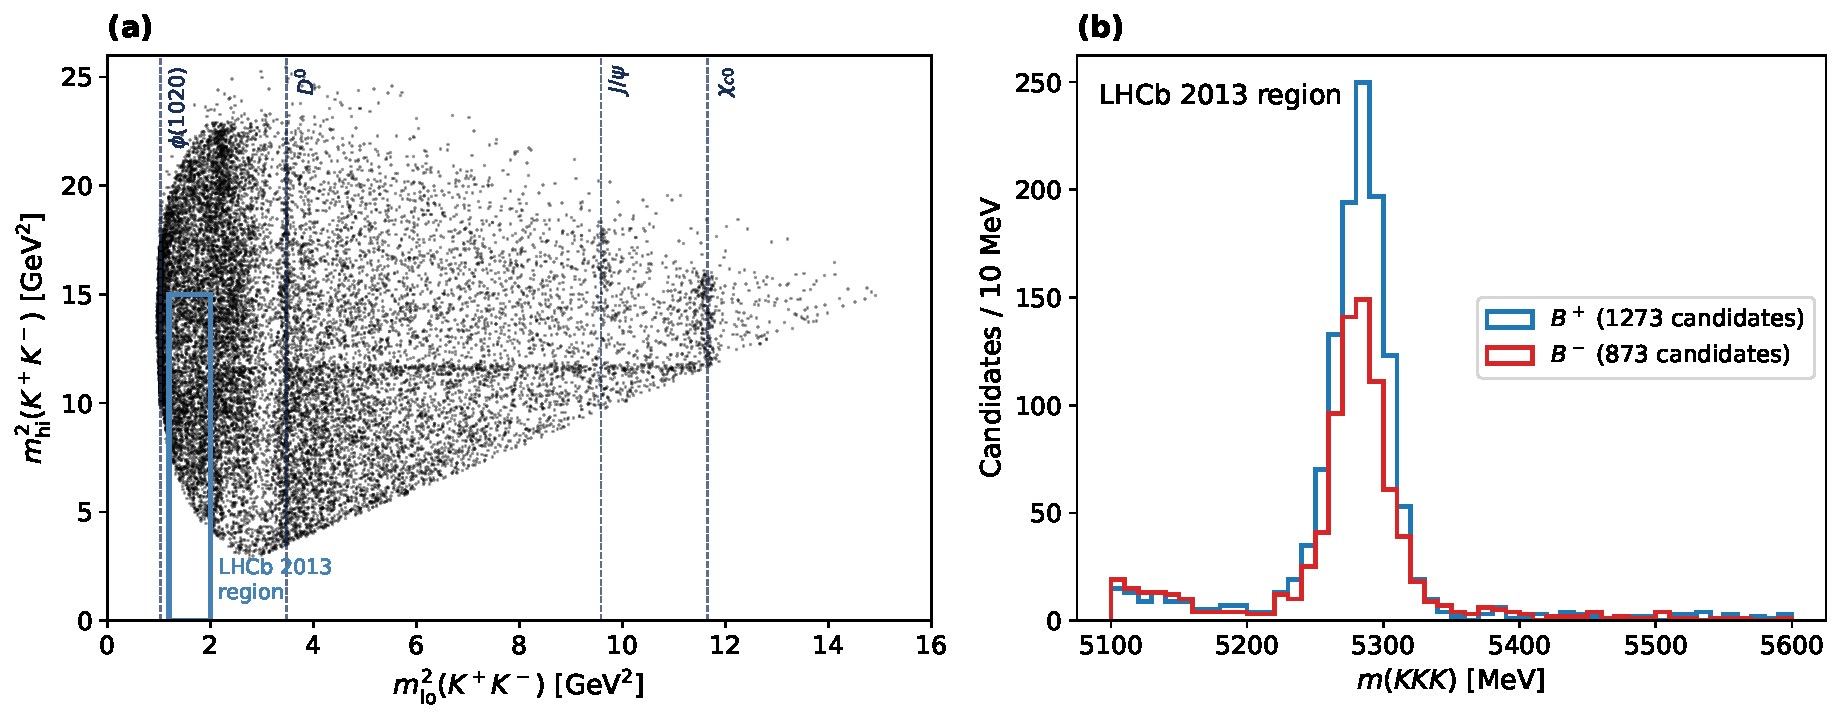
\includegraphics[width=0.95\textwidth]{figures/ml_nominal_dalitz_region.pdf}
\caption{(a) Ordered Dalitz plot of the candidates in the fit window, with the squared masses of the $\phi(1020)$, $D^0$, $J/\psi$ and $\chi_{c0}$ (dashed) and the region of the published analysis of the same data~\cite{lhcb_cpv_2013} (box). (b) Mass spectra of $B^+$ and $B^-$ candidates in that region, same binning: the $B^-$ peak is visibly smaller.}
\label{fig:dalitz_region}
\end{figure*}

Where is the asymmetry in terms of the decay dynamics? The ordered Dalitz plot (Fig.~\ref{fig:dalitz_region}a) shows the $\phi(1020)$ band at the kinematic edge ($m^2_{\mathrm{lo}}\approx1.04\,\GeV^2$) and the charm bands of the $D^0$, $J/\psi$ and $\chi_{c0}$. The negative asymmetry is not produced by the $\phi(1020)$: its band ($1964$ candidates) has $A_{\mathrm{count}}=-0.004\pm0.023$, while the significant bins without it have $-0.145\pm0.019$ (Fig.~\ref{fig:dalitz_phi} of Appendix~\ref{app:ext_dalitz}). It sits just above the $\phi$, where the published analysis located it, defining the region $1.2<m^2_{\mathrm{lo}}<2.0\,\GeV^2$, $m^2_{\mathrm{hi}}<15\,\GeV^2$ with $\Araw=-0.239\pm0.020$~\cite{lhcb_cpv_2013}. The region is fixed by the paper, not chosen on our data, so the comparison is unbiased: the nominal model fitted to its $2146$ candidates gives $\Araw=-0.234\pm0.025$ (Bayesian) and $-0.237\pm0.025$ (frequentist, $9.4\sigma$ from zero), reproducing the published value (spectra of the two charges in Fig.~\ref{fig:dalitz_region}b, where the $B^-$ peak is visibly smaller).

Three caveats limit the interpretation: the binning is coarse and was not optimized, the asymmetries are counts without sWeight background subtraction (Appendix~\ref{sec:limitations}), and local variations can be partly instrumental, since the $K^\pm$ interaction asymmetry depends on momenta that are correlated with the Dalitz position. In summary, the global asymmetry is not uniform over phase space, and the region identified by the published analysis carries it.




